\setcounter{chapter}{18}
\chapter{Lunette Astronomique}
\section{Constructions Fondamentales}
\subsection{Construction de l'image de l'objet AB}

\blocrouge{Vocabulaire et Règles}{
\begin{itemize}
\item O est le \trou{centre optique de la lentille.}
\item F est le \trou{foyer principal objet de la lentille.}
\item F' est le \trou{foyer principal image de la lentille.}
\item $OF=OF'$ désigne la distance focale en mètre. $v=\frac{1}{f'}$ est la vergence de la lentille en \trou{dioptrie noté : $\delta$}
\end{itemize}
\begin{enumerate}
	\item Tout rayon parallèle à l'axe optique émerge en \trou{passant par le foyer image F'}
	\item Tout rayon incident passant par le centre O émerge de la lentille \trou{sans être dévié.}
	\item Tout rayon incident passant par le foyer F émerge \trou{parallèlement à l'axe optique.}
\end{enumerate}
}

\etiquette{Schéma important}: Construction de l'image d'un objet AB par une lentille (L) 


\includegraphics{figures/lunette/rappel_1}

\etiquette{Consignes} En utilisant 3 rayons particuliers émis par B, construire son image B'. En déduire l'image A'B' produite par la lentille.

\subsection{Objet à l'infini}
Eloignons progressivement un point lumineux B et observons l'inclinaison des rayons qui entrent dans la lentille. \\

\includegraphics{figures/lunette/lunette_01}

On observe que plus B est loin de la lentille, plus l'angle entre les rayons qui pénètrent dans la lentille est petit. \\ A la limite lorsque B est infiniment à gauche sur la figure, cet angle devient nul  et les rayons qui pénètrent dans la lentille sont parallèles.

\blocrouge{Propriété 1}{
Un point \textbf{objet situé à l'infini} est représenté par une collection de \trou{\textbf{rayons lumineux parallèles} entre eux.}}

\etiquette{Construction 1} Objet B situé à \trou{l'infini}
\\
%version prof
%\includegraphics[scale=.75]{figures/lunette/lunette_02}
%version élève
\includegraphics{figures/lunette/lunette_03} 
\\
\etiquette{Stratégie de construction}: 
\begin{enumerate}
	\item Tracer le rayon passant par O
	\item Repérer l'intersection entre ce rayon et le plan focal: c'est B'
	\item Tous les rayons émis par $B_\infty$ sortent de la lentille en passant par B'
\end{enumerate}
\etiquetterouge{On retient} L'image d'un objet AB situé à l'infini est située dans \trou{\textbf{le plan focal image}} de la lentille.

\subsection{Objet situé dans le plan focal objet}
\etiquette{Construction 2}\\
%version prof
%\includegraphics[scale=.75]{figures/lunette/lunette_04}
%version élève
\includegraphics[scale=.75]{figures/lunette/lunette_05}
\\

\etiquette{Stratégie de construction}
\begin{enumerate}
	\item Tracer le rayon passant par O qui n'est pas dévié.
	\item Tracer le rayon émis par B et parallèle à l'axe optique, il sort en passant par F'
	\item Tous les rayons émis par B sortent de la lentille selon des rayons parallèles aux deux premiers tracés.
\end{enumerate}
\etiquetterouge{On retient} L'image d'un objet AB situé dans le plan focal objet de la lentille est situé à \textbf{l'infini}. C'est à dire que les rayons émergent \trou{parallèlement entre eux. } L'oeil voit dans le prolongement \trou{des rayons qu'il reçoit}.

\section{Présentation de la lunette astronomique}
\subsection*{Un peu d'histoire}
La lunette astronomique a été mise au point par Johannes Kepler en 1611 pour observer les astres ou les objets très éloignés. Il a repris la lunette de Galilée mise au point au siècle précédent et l'a améliorée.\\

\etiquette{Intérêt de la lunette}\\
La lunette astronomique a pour but d'observer des objets à l'infini, et de les grossir afin qu'ils soient observés par un \oe il sans accommodation (sans effort comme quand on regarde au loin). \\
Pour que l'\oe il n'accommode pas, l'image à la sortie de la lentille doit être formée à l'infini.\\
La lunette astronomique donne donc d'un objet à l'infini une image à l'infini, c'est ce que l'on appelle un dispositif \trou{afocal} (c'est à dire ne comportant pas de foyer).

\etiquette{Anatomie}\\
La lunette astronomique est constituée de \trou{Deux lentilles convergentes} :\\
\begin{minipage}{0,65\linewidth}
\begin{itemize}
\item \textbf{L'objectif} : Il se trouve du côté de \trou{l'objet} que l'on souhaite observer.\\
Il forme d'un objet $A_\infty B_\infty$ à l'infini une image $A_1B_1$ dans le plan focal image.\\
 Il est modélisé par une lentille convergente, notée $L_1$, de distance focale $f'_1$

\vspace{1,5cm}
\item \textbf{L'oculaire} : Il se trouve du côté de \trou{l'oeil}.\\
Il forme d'un objet $A_1B_1$ situé dans le plan focal objet une image à l'infini $A'_\infty B'_\infty$.\\
il est modélisé par une lentille convergente, de distance focale $f'_2$.
\end{itemize}
\end{minipage}
\begin{minipage}{0,3\linewidth}
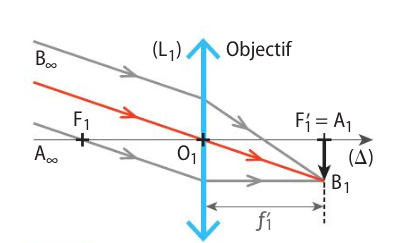
\includegraphics[scale=0.4]{figures/lunette/fig_obj}
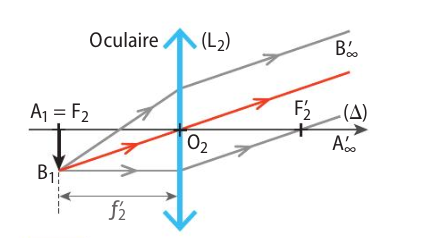
\includegraphics[scale=0.4]{figures/lunette/fig_oc}
\end{minipage}


Pour que la lunette soit afocale, il faut que \trou{le plan focal image de l'objectif} soit confondu avec \trou{le plan focal objet de l'oculaire.}\\

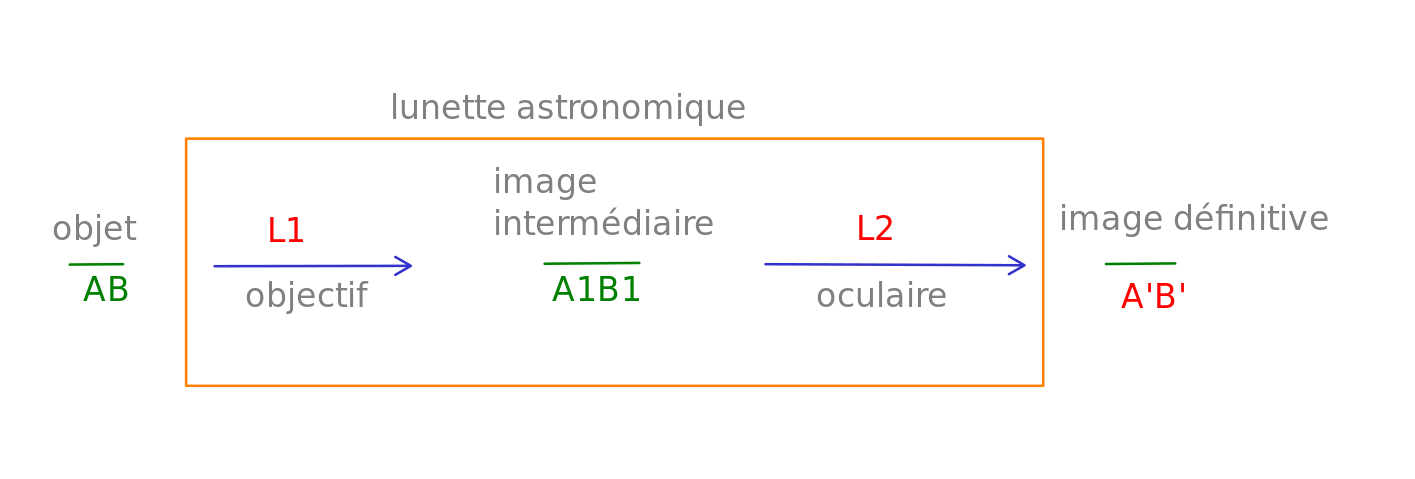
\includegraphics[scale=0.3]{figures/lunette/fig_modele}\\


\section{Construction du faisceau traversant une lunette afocale}
\etiquetterouge{Objectif} Tracer (sur le schéma incomplet qui suit)  le trajet des rayons émis par un objet AB situé à l'infini de la lentille. On doit obtenir la construction suivante:\\
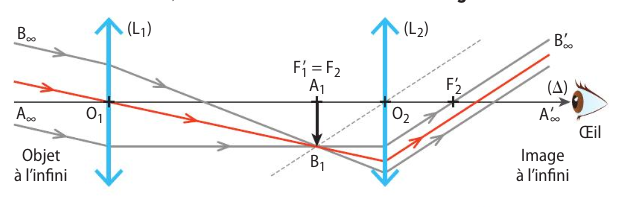
\includegraphics[scale=0.7]{figures/lunette/fig_lunette}\\
\includegraphics{figures/lunette/lunette_07}

%\newpage

\blocrouge{Entraînement à la Maison}{

Représenter, à l'échelle $\dfrac{1}{5}$ le modèle de la lunette astronomique suivante : \begin{itemize}
\item L'objectif est une lentille convergente de distance focale $f'_1=\SI{50}{\centi\meter}$
\item L'oculaire est une lentille convergente de distance focale $f'_2=\SI{10}{\centi\meter}$
\end{itemize}
Tracer le trajet de rayons lumineux issus d'un objet situé à l'infini, rayons faisant un angle $\alpha$ avec l'axe optique, à travers la lunette astronomique.\\ On notera $\alpha '$ l'angle fait par les rayons émergents avec l'axe optique.
}

\vspace{2cm}

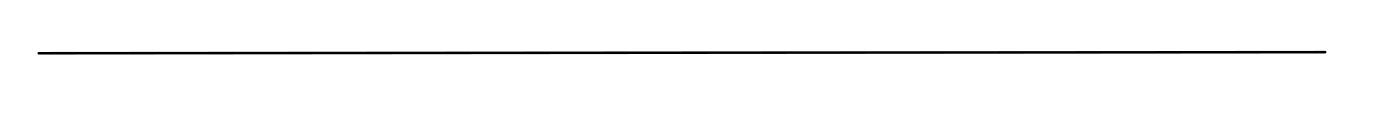
\includegraphics[scale=0.4]{figures/lunette/axe}

\vspace{2cm}
\newpage
\section{Grossissement}
\subsection{Grossissement G d'un système afocal}
Le grossissement noté G est une grandeur sans unité liée aux angles sous lesquels on observe l'objet à l'\oe il nu et son image à travers la lunette.\\

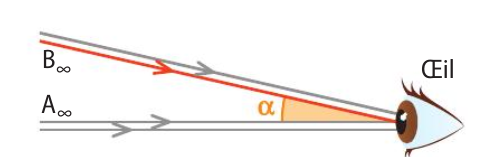
\includegraphics[scale=0.5]{figures/lunette/alpha}
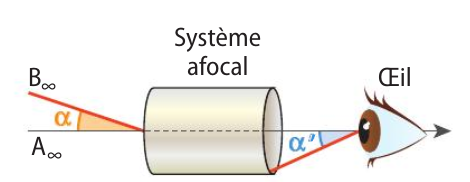
\includegraphics[scale=0.5]{figures/lunette/alpha'}\\
A travers la lunette, on voit l'astre comme s'il était situé à une distance plus petite que la distance réelle. Donc, l'angle $\alpha'$ est plus grand que l'angle $\alpha$.

\blocrouge{Définition}{
On définit le grossissement comme étant 
$$\trou{\boxed{G=\dfrac{\alpha'}{\alpha}}}$$

avec $\alpha'$ l'angle sous lequel l'image définitive A'B' est vue à travers la lunette\\
Et $\alpha$ l'angle sous lequel l'objet AB est vu à l'\oe il nu.
}


\subsection{Calcul de G pour la lunette astronomique}
\etiquette{Stratégie}
\begin{enumerate}
	\item Calculer $\tan\alpha$ et $\tan\alpha '$ dans un triangle dont un des côtés est $A_1B_1$.
	\item Faire l'approximation des petits angles: $\tan\alpha\approx\alpha$
	\item Calculer $G=\dfrac{\alpha '}{\alpha}$ 
\end{enumerate}
\begin{minipage}{0,4\linewidth}
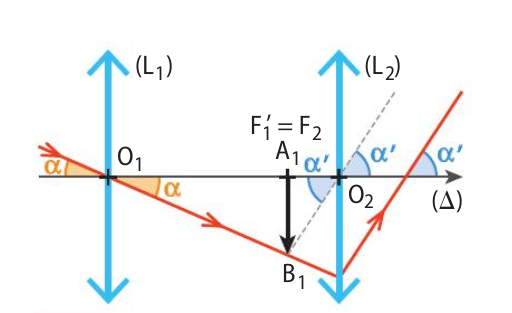
\includegraphics[scale=0.4]{figures/lunette/grossissement}
\end{minipage}
\begin{minipage}{0,6\linewidth}
Dans le triangle $O_1A_1B_1$, on a $\tan \alpha =$
\end{minipage}
\newpage
\etiquetterouge{Votre Synthèse}

\tikzset{every picture/.style={line width=0.75pt}} %set default line width to 0.75pt        

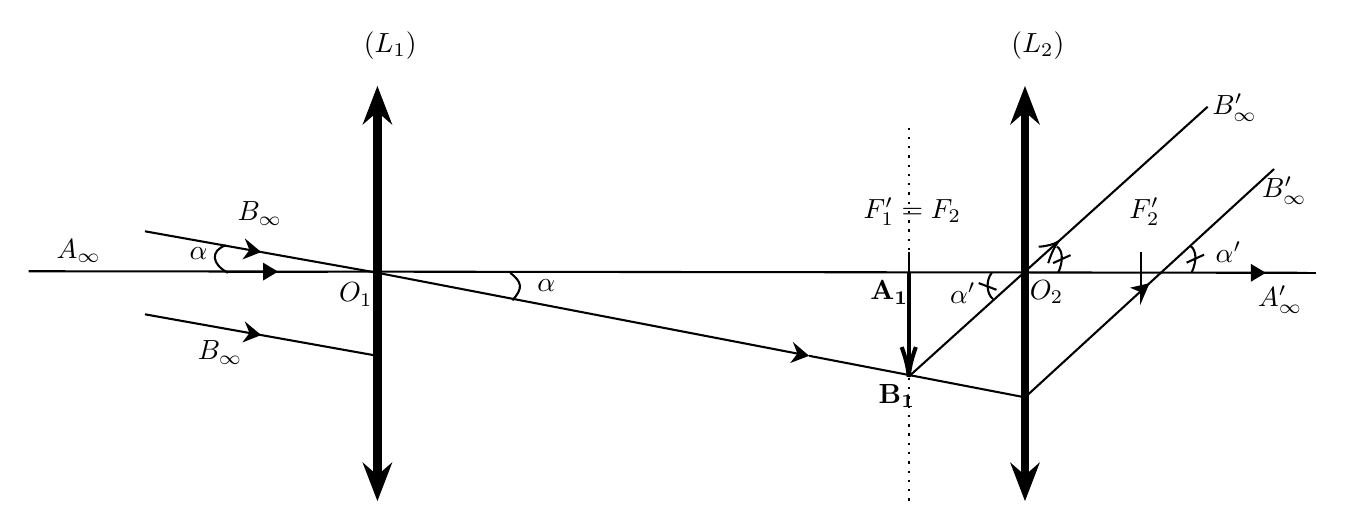
\begin{tikzpicture}[x=0.75pt,y=0.75pt,yscale=-1,xscale=.8]
%uncomment if require: \path (0,300); %set diagram left start at 0, and has height of 300

%Straight Lines [id:da2168956321390959] 
\draw    (-65,129.25) -- (705,130) ;
%Straight Lines [id:da11173057992958146] 
\draw [line width=3]    (145,46) -- (145,234) ;
\draw [shift={(145,240)}, rotate = 270] [fill={rgb, 255:red, 0; green, 0; blue, 0 }  ][line width=0.08]  [draw opacity=0] (18.75,-9.01) -- (0,0) -- (18.75,9.01) -- (12.45,0) -- cycle    ;
\draw [shift={(145,40)}, rotate = 90] [fill={rgb, 255:red, 0; green, 0; blue, 0 }  ][line width=0.08]  [draw opacity=0] (18.75,-9.01) -- (0,0) -- (18.75,9.01) -- (12.45,0) -- cycle    ;
%Straight Lines [id:da7566910966643488] 
\draw    (465,120) -- (465,140) ;
%Straight Lines [id:da6357288075561843] 
\draw [line width=3]    (535,46) -- (535,234) ;
\draw [shift={(535,240)}, rotate = 270] [fill={rgb, 255:red, 0; green, 0; blue, 0 }  ][line width=0.08]  [draw opacity=0] (18.75,-9.01) -- (0,0) -- (18.75,9.01) -- (12.45,0) -- cycle    ;
\draw [shift={(535,40)}, rotate = 90] [fill={rgb, 255:red, 0; green, 0; blue, 0 }  ][line width=0.08]  [draw opacity=0] (18.75,-9.01) -- (0,0) -- (18.75,9.01) -- (12.45,0) -- cycle    ;
%Straight Lines [id:da9852783124894242] 
\draw    (605,120) -- (605,140) ;
%Straight Lines [id:da3109976381088303] 
\draw    (275,150) -- (145,130) ;
%Straight Lines [id:da8566852525579076] 
\draw    (402.03,169.54) -- (275,150) ;
\draw [shift={(405,170)}, rotate = 188.75] [fill={rgb, 255:red, 0; green, 0; blue, 0 }  ][line width=0.08]  [draw opacity=0] (10.72,-5.15) -- (0,0) -- (10.72,5.15) -- (7.12,0) -- cycle    ;
%Straight Lines [id:da7648211303216299] 
\draw    (535,190) -- (405,170) ;
%Straight Lines [id:da35136732445197005] 
\draw  [dash pattern={on 0.84pt off 2.51pt}]  (465,60) -- (465,240) ;
%Straight Lines [id:da8597413149358359] 
\draw    (465,180) -- (645,50) ;
\draw [shift={(555,115)}, rotate = 144.16] [color={rgb, 255:red, 0; green, 0; blue, 0 }  ][line width=0.75]    (10.93,-4.9) .. controls (6.95,-2.3) and (3.31,-0.67) .. (0,0) .. controls (3.31,0.67) and (6.95,2.3) .. (10.93,4.9)   ;
%Straight Lines [id:da274094382380242] 
\draw    (535,190) -- (685,80) ;
\draw [shift={(610,135)}, rotate = 143.75] [fill={rgb, 255:red, 0; green, 0; blue, 0 }  ][line width=0.08]  [draw opacity=0] (10.72,-5.15) -- (0,0) -- (10.72,5.15) -- (7.12,0) -- cycle    ;
%Straight Lines [id:da847708984830482] 
\draw    (5,110) -- (145,130) ;
\draw [shift={(75,120)}, rotate = 188.13] [fill={rgb, 255:red, 0; green, 0; blue, 0 }  ][line width=0.08]  [draw opacity=0] (10.72,-5.15) -- (0,0) -- (10.72,5.15) -- (7.12,0) -- cycle    ;
%Straight Lines [id:da02702840130814277] 
\draw    (5,150) -- (145,170) ;
\draw [shift={(75,160)}, rotate = 188.13] [fill={rgb, 255:red, 0; green, 0; blue, 0 }  ][line width=0.08]  [draw opacity=0] (10.72,-5.15) -- (0,0) -- (10.72,5.15) -- (7.12,0) -- cycle    ;
%Curve Lines [id:da5961926220635629] 
\draw    (53.75,116.75) .. controls (44.33,119.22) and (45,125.89) .. (55,130) ;
%Curve Lines [id:da23585236461317316] 
\draw    (225,130) .. controls (231.75,134.25) and (233.25,137.25) .. (226.25,143.25) ;
%Straight Lines [id:da4781405060937802] 
\draw [line width=1.5]    (465,130) -- (465,177) ;
\draw [shift={(465,180)}, rotate = 270] [color={rgb, 255:red, 0; green, 0; blue, 0 }  ][line width=1.5]    (14.21,-4.28) .. controls (9.04,-1.82) and (4.3,-0.39) .. (0,0) .. controls (4.3,0.39) and (9.04,1.82) .. (14.21,4.28)   ;
%Curve Lines [id:da5186850592414963] 
\draw    (515,130) .. controls (511.36,133.55) and (511.73,140.18) .. (515.73,142.64) ;
\draw [shift={(512.49,136.58)}, rotate = 286.77] [color={rgb, 255:red, 0; green, 0; blue, 0 }  ][line width=0.75]    (0,5.59) -- (0,-5.59)   ;
%Curve Lines [id:da359362515174557] 
\draw    (554.27,117.36) .. controls (557.86,119.29) and (558.14,124.43) .. (555,130) ;
\draw [shift={(557.16,123.41)}, rotate = 249.91] [color={rgb, 255:red, 0; green, 0; blue, 0 }  ][line width=0.75]    (0,5.59) -- (0,-5.59)   ;
%Curve Lines [id:da2510289125381956] 
\draw    (634.71,117.14) .. controls (638.3,119.06) and (638.58,124.21) .. (635.44,129.78) ;
\draw [shift={(637.6,123.19)}, rotate = 249.91] [color={rgb, 255:red, 0; green, 0; blue, 0 }  ][line width=0.75]    (0,5.59) -- (0,-5.59)   ;
%Straight Lines [id:da10265543314732706] 
\draw    (55.14,129.43) -- (115.14,129.43) ;
\draw [shift={(85.14,129.43)}, rotate = 180] [fill={rgb, 255:red, 0; green, 0; blue, 0 }  ][line width=0.08]  [draw opacity=0] (8.93,-4.29) -- (0,0) -- (8.93,4.29) -- cycle    ;
%Straight Lines [id:da7876984232434279] 
\draw    (650,130) -- (710,130) ;
\draw [shift={(680,130)}, rotate = 180] [fill={rgb, 255:red, 0; green, 0; blue, 0 }  ][line width=0.08]  [draw opacity=0] (8.93,-4.29) -- (0,0) -- (8.93,4.29) -- cycle    ;

% Text Node
\draw (436,92.4) node [anchor=north west][inner sep=0.75pt]    {$F'_{1} =F_{2}$};
% Text Node
\draw (135,12.4) node [anchor=north west][inner sep=0.75pt]    {$( L_{1})$};
% Text Node
\draw (120,133.4) node [anchor=north west][inner sep=0.75pt]    {$O_{1}$};
% Text Node
\draw (536,132.4) node [anchor=north west][inner sep=0.75pt]    {$O_{2}$};
% Text Node
\draw (596,92.4) node [anchor=north west][inner sep=0.75pt]    {$F'_{2}$};
% Text Node
\draw (525,12.4) node [anchor=north west][inner sep=0.75pt]    {$( L_{2})$};
% Text Node
\draw (59,94.4) node [anchor=north west][inner sep=0.75pt]    {$B_{\infty }$};
% Text Node
\draw (35,161.4) node [anchor=north west][inner sep=0.75pt]    {$B_{\infty }$};
% Text Node
\draw (30,116.4) node [anchor=north west][inner sep=0.75pt]    {$\alpha $};
% Text Node
\draw (239.5,131.9) node [anchor=north west][inner sep=0.75pt]    {$\alpha $};
% Text Node
\draw (445,182.4) node [anchor=north west][inner sep=0.75pt]    {$\mathbf{B_{1}}$};
% Text Node
\draw (440,132.4) node [anchor=north west][inner sep=0.75pt]    {$\mathbf{A_{1}}$};
% Text Node
\draw (488,133.4) node [anchor=north west][inner sep=0.75pt]    {$\alpha '$};
% Text Node
\draw (648,113.4) node [anchor=north west][inner sep=0.75pt]    {$\alpha '$};
% Text Node
\draw (646,42.4) node [anchor=north west][inner sep=0.75pt]    {$B'_{\infty }$};
% Text Node
\draw (676,82.4) node [anchor=north west][inner sep=0.75pt]    {$B'_{\infty }$};
% Text Node
\draw (-50,112.4) node [anchor=north west][inner sep=0.75pt]    {$A_{\infty }$};
% Text Node
\draw (673.5,134.9) node [anchor=north west][inner sep=0.75pt]    {$A'_{\infty }$};


\end{tikzpicture}


\etiquetterouge{Exercices}

\begin{itemize}
	\item Reconnaître le montage: 2, 3 p 396
	\item Tracer des rayons: 5, 6 , 9 p 397
	\item Calculs classiques: 11 et 12 p 398
	\item Préparer le bac: 24, 25 p 403
 	\item TYPE BAC: \url{https://labolycee.org/observation-ornithologique-dune-oie-cendree}
\end{itemize}